\documentclass{article}

\usepackage{Vor2017skil}

\title{Tölvunarfræði 2, \semester \\ Skilaverkefni 11}
\author{}

\begin{document}
\maketitle
\hypersetup{pdftitle={Tölvunarfræði 2 - Skilaverkefni 11}}

\paragraph{Skilavefur} Skila skal þessum verkefnum á \href{https://gradescope.com/courses/5640}{Gradescope}.

\paragraph{Vinnubrögð og frágangur} Skrifa þarf forrit í Java og C++ sem útfæra ýmsar aðferðir. Í öllum tilvikum skal skila \texttt{main} fall/aðferð sem býr til prufugögn og sýnir virkni hverrar aðferðar um sig. Skilið öllum forritskóða og sýnið dæmi um keyrslu. Leitist við að nota beinagrindur óbreyttar þegar þær eru gefnar. Vönduð framsetning og læsilegur kóði er hluti af verkefninu, sjá \href{https://piazza.com/class/ixkicfen49l111?cid=52}{glósu um frágang og framsetningu}.

\paragraph{Samþykki til dreifingar} Dæmatímakennarar velja framúrskarandi lausnir til birtingar undir nafni í lausnasafni. Sé þess óskað að einhverjar þinna úrlausna séu ekki birtar nema nafnlaust eða alls ekki birtar yfir höfuð skal taka slíkt fram í hverju dæmi sem takmörkunin á við.

\section{Spurning 1}
Skrifið forrit sem finnur og skrifar út þyngdina á léttasta spanntré í \href{https://github.com/Ernir/kennsluefni/tree/master/T2/Code/w11/tinyEWG.txt}{tinyEWG.txt}.

\section{Spurning 2}
Hægt er að útfæra net með ýmsum hætti. Í stað þess að búa til sérstakan klasa til að tákna net gætum við ákveðið að nota innbyggðar gagnagrindur.

T.d. mætti nota \texttt{std::map} í C++ til að halda utan um net með því að nota númer hnúta sem lykla og láta gildin vera \texttt{std::vector} af númerum nágranna hvers hnúts:

\begin{minted}[frame=lines]{cpp}
map<int, vector<int>> tinyG;
// Skilgreint að hnútur með númerið 4 hafi nágrannana 2 og 3
tinyG.insert(make_pair(4, vector<int>({2, 3})));
\end{minted}

En til þess að vinna með gögn sem geymd eru á lauslega skilgreindan máta þarf góð reiknirit.

Skrifið \texttt{displayGraph} fall í C++, sem tekur inn stefnt net táknað með svipuðum hætti og í dæminu hér að ofan og skrifar það út á skipanalínuna. Snið útskriftarinnar á að vera það sama og \texttt{toString()} aðferð \texttt{DiGraph} klasans notar. 

Sýnið dæmi um keyrslu þar sem netið sem skilgreint er í \href{https://github.com/Ernir/kennsluefni/tree/master/T2/Code/w10/tinyDG.txt}{tinyDG.txt} er skrifað út. Það ætti að vera:

\begin{verbatim}
0: 5 1 
1: 
2: 0 3 
3: 5 2 
4: 3 2 
5: 4 
6: 9 4 8 0 
7: 6 9 
8: 6 
9: 11 10 
10: 12 
11: 4 12 
12: 9
\end{verbatim}

Notið beinagrindina í \href{https://github.com/Ernir/kennsluefni/tree/master/T2/Code/w11/mapgraph.cpp}{mapgraph.cpp}.

\paragraph{Ábending:} Gagnlegt gæti verið að skoða C++ sýnidæmi úr 3. kennsluviku.

% \section{Spurning 2}map<string, vector<string>> courses;
% Eftirfarandi tafla er af gömlu vegakorti. Hún er sögð innihalda stystu leiðir á milli nokkurra borga, en hún inniheldur villu.
% \begin{center}
% \includegraphics[width=0.8\textwidth]{shortest-routes}
% \end{center}
% Finnið villuna. Skrifið forrit sem notar netareiknirit til að lagfæra töfluna.

\section{Spurning 3}
Klassískt netavandamál er að finna leið í gegnum völundarhús. Til að gera það má skipta völundarhúsinu upp í reiti, þar sem hver reitur er táknaður með hnúti. Sé mögulegt að stíga af einum reit á annan táknum við það með legg á milli hnútanna. 

Ef við notum vegið örvanet til að tákna völundarhúsið getum við gert greinarmun á erfiðum leiðum og auðveldum leiðum.

Skráin \href{https://github.com/Ernir/kennsluefni/tree/master/T2/Code/w11/maze.txt}{maze.txt} táknar völundarhús með því að nota nokkur tákn. Merkingar táknanna eru eftirfarandi:
\begin{itemize}
 \item \texttt{-} venjulegur reitur. Hægt er að stíga á slíkan reit af reitunum sem eru fyrir norðan, sunnan, austan eða vestan hann.
 \item \texttt{=} sleipur reitur. Hægt er að stíga á hann eins og venjulegan reit, en það er tvöfalt erfiðara.
 \item \texttt{I} inngangur. Venjulegur reitur sem við byrjum í.
 \item \texttt{U} útgangur. Venjulegur reitur sem við viljum komast á.
 \item \texttt{X} óaðgengilegur reitur (veggir).
\end{itemize}

Látið örvalegg sem stefnir á hnút sem táknar venjulegan reit hafa þyngdina 1, en örvalegg sem stefnir á hnút sem táknar sleipan reit hafa þyngdina 2. Skrifið Java-forrit sem les inn \texttt{maze.txt} og skrifar út léttustu leið í gegnum völundarhúsið.

Þetta verkefni má leysa á nokkuð marga vegu. Ekki er gefin beinagrind.

\section{Spurning 4}
Skjalið \href{https://github.com/Ernir/kennsluefni/tree/master/T2/Code/w11/qatar.txt}{qatar.txt}\footnote{Uppruni: \url{http://www.math.uwaterloo.ca/tsp/world/countries.html}} inniheldur staðsetningar (hnit) á þéttbýlissvæðum í smáríkinu Katar.

Gefum okkur nú að Katar vilji skipta út rafmagnsdreifikerfi sínu þannig að nýja kerfið myndi léttasta mögulega evklíðskt spanntré (e.\ \emph{Euclidean minimum spanning tree}) í neti sem myndað er út frá staðsetningunum. Þegar mynda skal slíkt tré lítum við á sem svo að mögulegt væri að bæta við legg á milli hverra tveggja hnúta (staðsetninga), þar sem þyngd leggsins er fjarlægðin á milli hnútanna.

Skrifið forrit í Java sem reiknar út léttasta evklíðska spanntré í Katar-netinu, skrifar út heildarþyngd þess og teiknar það. Notið beinagrindina í \href{https://github.com/Ernir/kennsluefni/tree/master/T2/Code/w11/Qatar.java}{Qatar.java}.

\begin{figure}[h]
\caption{Hnitin í Katar-netinu}
\begin{center}
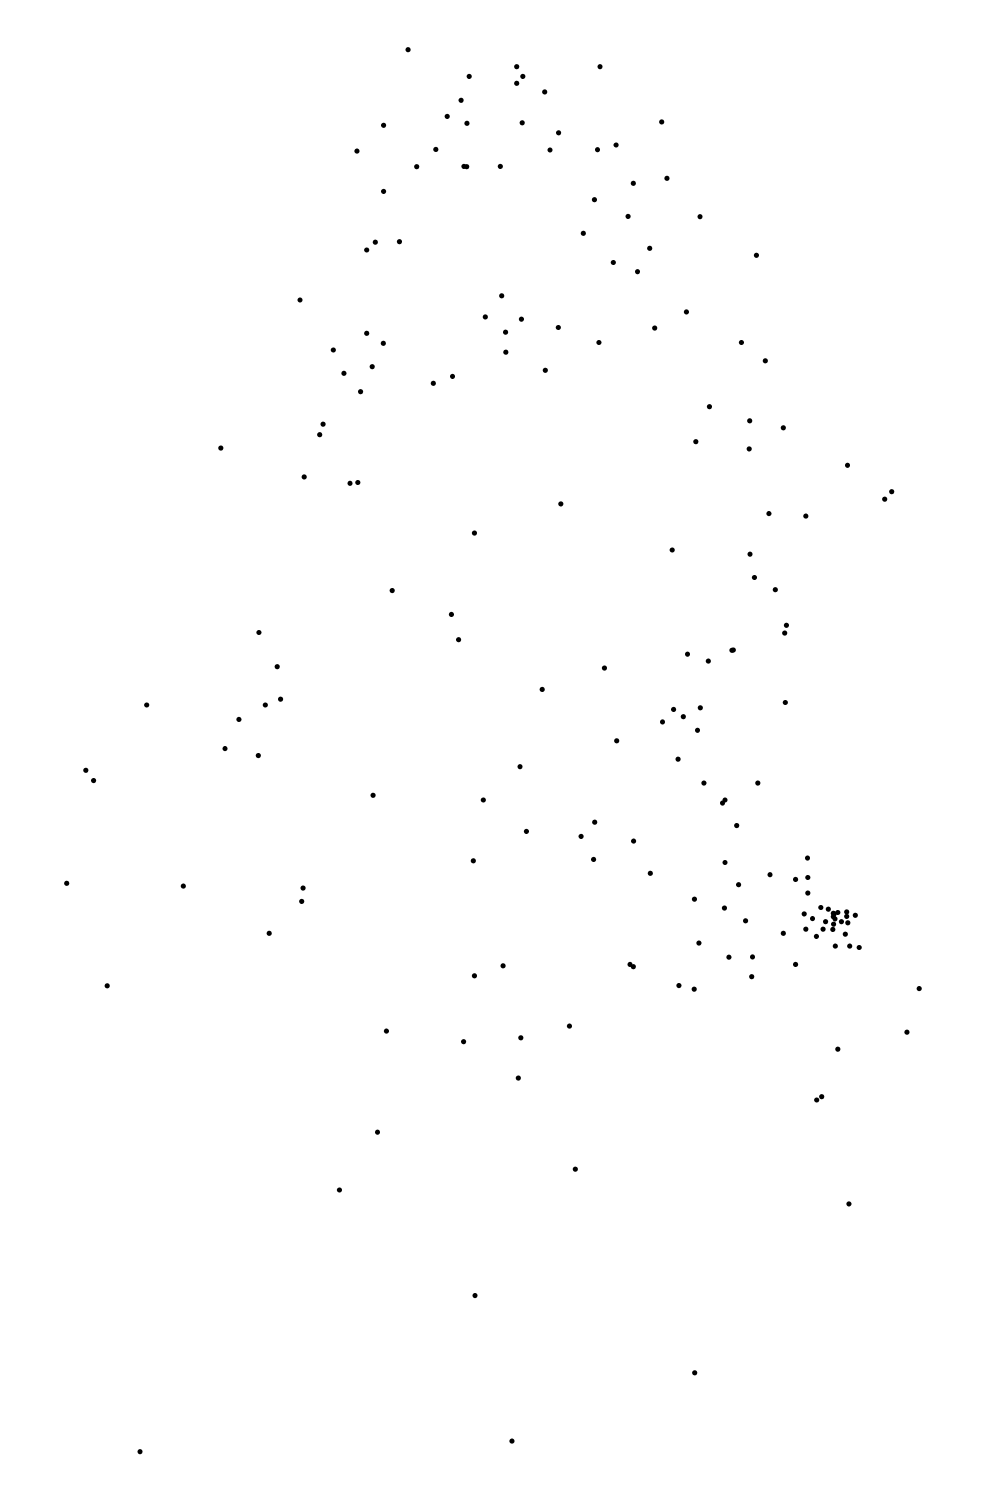
\includegraphics[width=0.8\textwidth]{qatar}
\end{center}
\end{figure}

\begin{figure}
\caption{Spanntré kennarans, með heildarþyngdina 8028.0137422378375}
\begin{center}
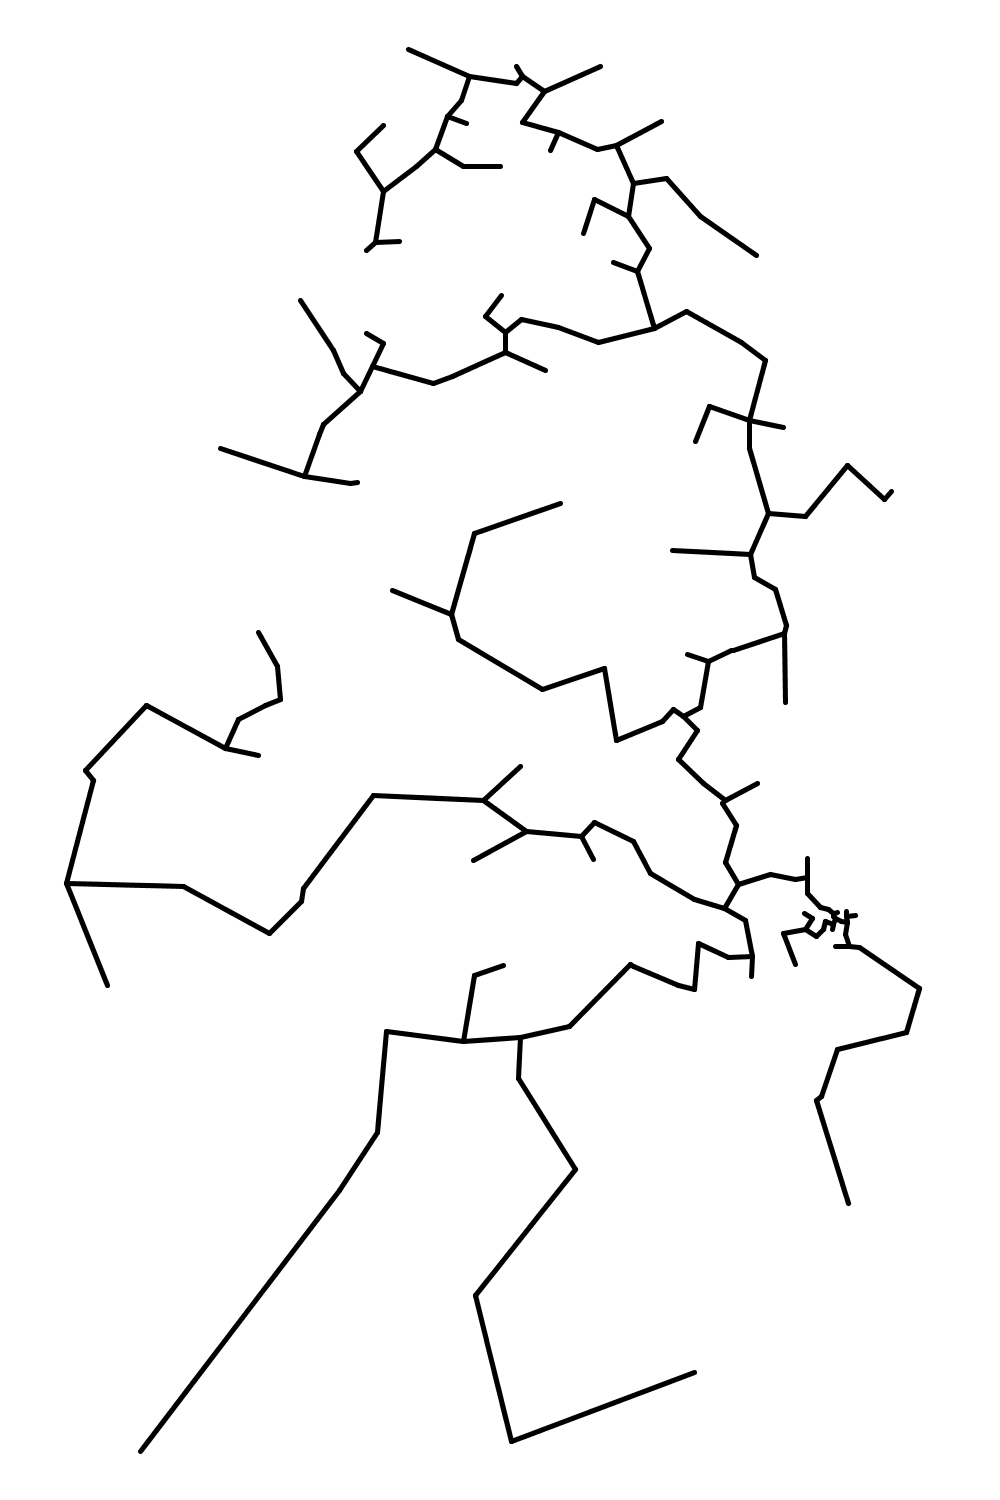
\includegraphics[width=0.8\textwidth]{qatar-mst}
\end{center}
\end{figure}

%\vfill
%
\includegraphics[width=0.5\linewidth]{hi-von-logo}
\end{document}